\documentclass{extarticle}
    \usepackage{graphicx}
	\usepackage{xcolor}
    \usepackage{geometry}        
		\geometry{
			papersize={42mm,153mm},
			total={42mm,153mm},
			top=0mm,
			left=0mm, 
		}     
    \newlength{\temph}
    \setlength{\unitlength}{1mm}
    \usepackage[{absolute,overlay}]{textpos}
    \TPGrid[0mm,0mm]{42}{153}
    
    \begin{filecontents}{\jobname.xmpdata}
    \Keywords{blok\sepšifrovací pomůcky}
    \Title{Šifrovací pomůcky} 
    \Author{Organizátoři hry Navíc}
    \end{filecontents}
    
\begin{document}
\pagecolor{black}
\pagestyle{empty}

\begin{textblock}{38}(2,2)
\vfill
{\centerline{
\includegraphics[width=38mm]{tools/numbers-table-v3.pdf}}} 
\vfill
\end{textblock}


\begin{textblock}{38}(2,94)
\vfill
{\centerline{
\includegraphics[scale=0.6333]{tools/keyboard-v2.pdf}}} 
\vfill
\end{textblock}

\begin{textblock}{38}(2,109)
\vfill
{\centerline{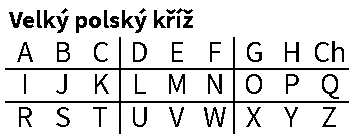
\includegraphics[scale=0.6333]{tools/rosicrucian-polish.pdf}}} 
\vfill
\end{textblock}

\begin{textblock}{26.6}(2,125)
\vfill
{\centerline{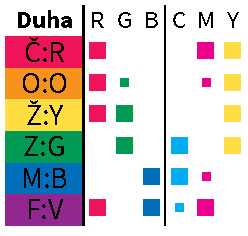
\includegraphics[scale=0.6333]{tools/rainbow-v2.pdf}}} 
\vfill
\end{textblock}

\begin{textblock}{0}(35,126)
\vfill
{\centerline{
\includegraphics[height=14mm]{tools/images/segment-numbering.pdf}}} 
\vfill
\end{textblock}


\end{document}

